%\documentclass[fleqn]{book}
\documentclass[11pt]{amsbook}

\usepackage[turkish]{babel}

%\usepackage{../HBSuerDemir}	% ------------------------
\usepackage{../Ceyhun}	% ------------------------
\usepackage{../amsTurkish}


\begin{document}
% ++++++++++++++++++++++++++++++++++++++
\hPage{152}
% ++++++++++++++++++++++++++++++++++++++
\begin{figure}[htb]
	\centering
	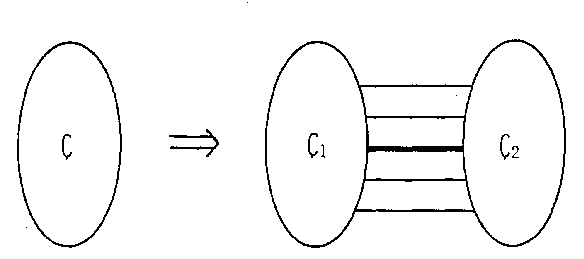
\includegraphics[width=0.45\textwidth]{images/ceyhun-152-fig01}
	\caption{H-matrisinin açıklanması}
\end{figure}
\par 
böylesine bir durum görülecektir. Yalnız $H(i)$ matrisinin iki altmatrise parçalanmasının her zaman için birlik olmadığı gözden kaçmamalıdır. Şekil 3.4.3 deki çizgenin t-kesitleme matrisi,
$$ Q_t = 
\begin{bmatrix}
1 & 0 & 0 & 0 & 0 & 0 & 1 & 1 \\
0 & 1 & 0 & 0 & 0 & 1 & 1 & 1 \\
0 & 0 & 1 & 0 & 0 & 1 & 1 & 1 \\
0 & 0 & 0 & 1 & 0 & 1 & 1 & 1 \\
0 & 0 & 0 & 0 & 1 & 1 & 0 & 1\\
\end{bmatrix} $$ 


\end{document}